\subsection{Dinamična geometrija z GeoGebro}

V poglavju \href{/geogebrauvod}{GeoGebra: Uvod} smo spoznali osnove dela z GeoGebro. V tem poglavju bomo raziskali, kako ustvariti animacije in dinamične konstrukcije z uporabo GeoGebre.

\subsubsection{Točka na objektu}

Najlažje način za ustvarjanje dinamične konstrukcije je uporaba točke, ki je vezana na drug objekt. Točko lahko postavimo na premico, krožnico ali katerikoli drug objekt, kar omogoča, da se točka premika znotraj omejitve tega objekta.

Ko ustvarimo točko na krivulji (kot so premice, krožnice, graf funkcij itd.), lahko to točko animiramo. To naredimo tako, da izberemo točko in kliknemo na gumb 
\includegraphics[width=0.02\linewidth]{files/18px-Nav_play_circle-74635dc1a7e6d0a614249108e021d156.png}

 \textit{Play} v algebrskem oknu ali uporabimo ukaz \texttt{StartAnimation(\textless točka\textgreater )}. S tem se bo točka začela premikati po objektu, na katerem je bila ustvarjena.

Na žalost GeoGebra ne omogoča animacije točk na daljših objektih, kot so mnogokotniki. Vendar pa lahko ustvarimo drsnike, ki nam omogočajo nadzor nad položajem točke na takšnih objektih s pomočjo parametra.

\subsubsection{Drsniki}

V resnični, drsniki so samo orodja za spreminjanje vrednosti spremenljivk. Vendar pa so zelo uporabni pri ustvarjanju dinamičnih konstrukcij, saj nam omogočajo, da spreminjamo vrednosti in opazujemo, kako se konstrukcija spreminja.

Drsniki imajo tri glavne lastnosti: \texttt{Min} (minimalna vrednost), \texttt{Max} (maksimalna vrednost) in \texttt{Increment} (prirastek). Te lastnosti določajo obseg vrednosti, ki jih drsnik lahko zavzame, in kako hitro se vrednost spreminja, ko premikamo drsnik.

Za ustvarjanje drsnika lahko uporabimo orodje 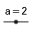
\includegraphics[width=0.0275\linewidth]{files/32px-Mode_slider.svg-e15eadebbb4f9101af436526f2609a2c.png}

 \textit{Slider} (\textit{Drsnik}) in dobimo okno za nastavitev lastnosti drsnika. Drsnike lahko ustvarimo tudi z vnosom imena spremenljivke v vnosno vrstico, na primer \texttt{a=5}, kar ustvari spremenljivk z imenom \texttt{a} in začetno vrednostjo 5. Nato lahko kliknemo na tri pike poleg imena spremenljivke v algebrskem oknu in nato \textit{Create slider} (\textit{Ustvari drsnik}). To ustvari drsnik z privzetimi lastnostmi (\texttt{Min=-5}, \texttt{Max=5}, \texttt{Increment=0.1}), ki jih lahko spremenimo z dvojnim klikom na drsnik (v grafičnem pogledu) ali z desnim klikom na ime spremenljivke v algebrskem oknu in izbiro \textit{Settings} (\textit{Nastavitve}). V oknu z nastavitvami lahko spremenimo lastnosti drsnika, kot so \texttt{Min}, \texttt{Max} in \texttt{Increment}, in tudi druge lastnosti, kot so barva, slog in vidnost.

Drsniki lahko tudi uporabimo za ustvarjanje animacij. To naredimo tako, da izberemo drsnik in kliknemo na gumb 
\includegraphics[width=0.02\linewidth]{files/18px-Nav_play_circle-74635dc1a7e6d0a614249108e021d156.png}

 \textit{Play} v algebrskem oknu ali uporabimo ukaz \texttt{StartAnimation(\textless drsnik\textgreater )}. S tem se bo vrednost drsnika začela spreminjati samodejno z določenim prirastkom, kar omogoča ustvarjanje animacij v konstrukciji.

\subsubsection{Zaporedja}

Ukaz \texttt{Sequence()} omogoča ustvarjanje zaporedij objektov v GeoGebri. Splošna oblika ukaza je \texttt{Sequence(\textless izraz\textgreater , \textless spremenljivka\textgreater , \textless začetek\textgreater , \textless konec\textgreater , \textless korak\textgreater )}, kjer \texttt{\textless izraz\textgreater } je izraz (običajno ukaz GeoGebre), ki ga želimo ponoviti, \texttt{\textless spremenljivka\textgreater } je spremenljivka, ki se spreminja v zaporedju, \texttt{\textless začetek\textgreater } in \texttt{\textless konec\textgreater } določata obseg vrednosti za spremenljivko, in \texttt{\textless korak\textgreater } določa, za koliko se spremenljivka poveča v vsakem koraku.
Variantne ukaza so:

\begin{itemize}
\item \texttt{Sequence(\textless konec\textgreater )} - ustvari zaporedje števil od 1 do \texttt{\textless konec\textgreater }.
\item \texttt{Sequence(\textless začetek\textgreater ,\textless konec\textgreater )} - ustvari zaporedje števil od \texttt{\textless začetek\textgreater } do \texttt{\textless konec\textgreater }.
\item \texttt{Sequence(\textless izraz\textgreater , \textless spremenljivka\textgreater , \textless začetek\textgreater , \textless konec\textgreater )} - ustvari zaporedje z privzetim korakom 1.
\end{itemize}

Ukaz \texttt{Sequence()} ustvari zaporedje objektov, če hočemo izbrati posamezne objekte iz zaporedja, lahko uporabimo ukaz\texttt{Element(\textless zaporedje\textgreater , \textless indeks\textgreater )}, kjer \texttt{\textless zaporedje\textgreater } je zaporedje objektov in \texttt{\textless indeks\textgreater } je indeks objekta, ki ga želimo izbrati (indeksi se začnejo pri 1).

Če hočemo izgraditi več objektov (namesto zaporedje objektov), lahko uporabimo naslednje način:

\begin{itemize}
\item Ustvarimo zaporedje objektov z ukazom \texttt{Sequence()}, npr. \texttt{kroznice = Sequence(Circle((0,0), i), i, 1, 5)}, ki ustvari zaporedje krožnic s polmeri od 1 do 5.
\item Nato uporabimo ukazi \texttt{Sequence()} in \texttt{Element()} za ustvarjanje zaporedja ukazov, npr. \texttt{kroU=Sequence("K\_\{"+i+"\} = Element(kroznice, "+i+")", i, 1, 5)}, ki ustvari zaporedje ukazov za vsako krožnico v zaporedju z imenom \texttt{krogU}. V tem primeru ustvarimo ukaze \texttt{K\_\{1\} = Element(kroznice, 1)}, \texttt{K\_\{2\} = Element(kroznice, 2)}, itd.
\item Na koncu uporabimo ukaz \texttt{Execute()} za izvedbo vsakega ukaza.
\end{itemize}

Ta način lahko uporabimo za ustvarjanje zaporedje ukazov, da ni nujno ustvariti objekte. Na primer z ukazom
\texttt{barv=Sequence("SetDynamicColor(L\_\{"+i+"\}, random(), random(), random(), 0.5)", i, 1, 40)}, ustvarimo zaporedje ukazov za nastavitev naključne barve za vsako daljico, nato pa z ukazom \texttt{Execute(barv)} izvedemo te ukaze in tako nastavimo barve za vse daljice naenkrat. \textit{Pozkusite to sami}!


\bigskip
\centerline{\rule{13cm}{0.4pt}}
\bigskip

Zaporedje in drsniki postanejo zelo močna orodja, ko jih kombiniramo skupaj. Na primer, lahko ustvarimo drsnik, ki določa število objektov v zaporedju, in nato uporabimo ta drsnik za ustvarjanje dinamične konstrukcije, ki se spreminja glede na vrednost drsnika. Ta način bomo raziskali v naslednjih vajah.

\subsubsection{Vaje}\label{08_geogebraDinGeometrija_vaje}

\begin{itemize}
\item Exercise~\ref{ex-paralelogram} - Ustvarite dinamični paralelogram in opazujte, kako se spreminja njegova površina.
\item Exercise~\ref{ex-drsniki-1} - Ustvarite premico z drsniki za naklon in presečišče z osjo y ter opazujte, kako se spreminja premica.
\item Exercise~\ref{ex-drsniki-2} - Ustvarite dinamično konstrukcijo, ki prikazuje veljavnost trikotne neenakosti s pomočjo drsnikov in dinamičnih barv.
\item Exercise~\ref{ex-drsniki-3} - Ustvarite animacijo z uporabo drsnikov za premikanje točk v ravnini.
\item Exercise~\ref{ex-drsniki-4} - Ustvarite dinamično konstrukcijo za seštevanje dveh celih števil z uporabo drsnikov.
\item Exercise~\ref{ex_sequences-1} - Ustvarite zaporedje točk na krožnici z uporabo ukaza \texttt{Sequence()}.
\item Exercise~\ref{ex_sequences-2} - Uporabite ukaz \texttt{Sequence()} za ustvarjanje vzorca premic v GeoGebri.
\item Exercise~\ref{ex_sequences-3} - Uporabite ukazi \texttt{Element()} in \texttt{Execute()} za ustvarjanje posamezni objektov iz zaporedje.
\end{itemize}

%  - [Vaje %s](#ex_sequences-4) - Ustvarite dinamično konstrukcijo za množenje dveh celih števil z uporabo drsnikov in ukaza `Sequence()`.

%  - [Vaje %s](#ex_pythagoras) - Ustvarite konstrukcijo, ki prikazuje dokaz Pitagorovega izreka z uporabo drsnikov.

%  - [Vaje %s](#ex-circleArea) - Ustvarite dinamično konstrukcijo za izračun površine kroga s pomočjo drsnika za polmer kroga.

%  :::{solution} ex_sequences-4
% :class: tip dropdown
% Lahko uporabite naslednje korake za ustvarjanje te konstrukcije:
% 1. Ustvarite drsnika `a` in `b` z lastnostmi: `Min=1`, `Max=10`, `Increment=1`.
% 2. Upoštevajte da ukaz `Sequence((i,j),i,1,a)` ustvari zaporedje točk v dani vrstici z drugim koordinato `j`. 
% 3. Uporabite ukaz `točke=Sequence(Sequence((i,j),i,1,a),j,1,b)` za ustvarjanje zaporedja točk v pravokotniku z dolžino `a` in širino `b`.
% 5. Z uporabo ukaza `FormulaText("$"+a+"\times"+b+"="+(a*b)+"$")` ustvarite dinamično besedilo, ki prikazuje rezultat množenja `a` in `b`.
% 6. Uredite položaj besedila in slog po želji.
% 
% Lahko odprete to konstrukcijo v GeoGebri [tukaj](https://www.geogebra.org/classic/nkczhbrd).
% 
% :::